\chapter{実対称行列の対角化}
\lectureinfo{2015年11月25日 1限}

\section{事務連絡}

そろそろ授業が全て終わります。それに向けて、何点か事務連絡です。
\begin{itemize}
\item 12/16に提出された答案とその解答は、レポートボックスにて返却します。
\item 添削済みの答案を受け取っていない人がかなりいます。自分の分をきちんと受け取ってください。また、お友達の分を見つけた人は、ぜひ持って行ってあげてください。ご協力お願いします。
\end{itemize}

\section{直交行列とGram--Schmidtの正規直交化法}

今回は実対称行列を対角化する方法を学びます。一般に固有多項式が重根を持ってしまうと、必ずしも行列が対角化可能でなく、対角成分のすぐ上に$1$がいくつか並んだJordan標準形が登場するのでした。ですがターゲットの行列が実対称行列の場合、固有多項式が重根を持ったとしても必ず対角化ができ、しかも対角化するための行列として正規直交基底が取れるのです。

\subsection{直交行列と正規直交基底}

最初に、直交行列について復習しておきましょう。$n$次正方行列$P \in \Mat_n(\mathbb{R})$が${}^t P P = I$、言い換えれば$P^{-1} = {}^tP$を満たすとき、$P$は\textbf{直交行列}であると言うのでした。直交行列$P$を列ベクトルの並びで$P = (\bm{p}_1 \ \bm{p}_2 \ \cdots \ \bm{p}_n)$と表すと、直交行列の条件${}^tP = P$は内積によって$\bm{p}_i \cdot \bm{p}_j = \delta_{ij}$と表せます。つまり$\bm{p}_1, \bm{p}_2, \ldots, \bm{p}_n$はどれも長さが$1$で、相異なる$2$本の列ベクトルはどれも直交します。また、この状況で$(\bm{p}_1, \bm{p}_2, \ldots, \bm{p}_n)$は$\mathbb{R}^n$の基底をなすことも分かります。こういう、標準基底のように$\bm{p}_i \cdot \bm{p}_j = \delta_{ij}$を満たす良い基底のことを、$\mathbb{R}^n$の\textbf{正規直交基底}といいます。

内積を用いて直交行列を特徴づける方法も思い出しておきましょう。$\mathbb{R}^n$の内積は$\bm{u} \cdot \bm{v} := {}^t\bm{u} \bm{v}$で定義されていました。よって$P$が直交行列なら、$(P\bm{u}) \cdot (P\bm{v}) = {}^t\bm{u}\, {}^tP P \bm{v} = {}^t\bm{u} \bm{v} = \bm{u} \cdot \bm{v}$です。逆に任意のベクトル$\bm{u}, \bm{v}$について$(P\bm{u}) \cdot (P\bm{v}) = \bm{u} \cdot \bm{v}$なら、特に$\bm{u} = \bm{e}_i$, $\bm{v} = \bm{e}_j$とすることで$\delta_{ij} = \bm{e}_i \cdot \bm{e}_j = (P\bm{e}_i) \cdot (P\bm{e}_j) = {}^t\bm{e}_i\, {}^tP P \bm{e}_j = ({}^tP P)_{ij}$が得られ、${}^tP P = I$だと分かります。直交行列であることは、標準内積を保つことと同値です。

\subsection{Gram--Schmidtの正規直交化法}

本題のGram--Schmidtの正規直交化法の話に入ります。$\mathbb{R}^n$の基底の中には、正規直交基底でないものもたくさんあります。ところが\textbf{どんな基底を持ってきても、そこから正規直交基底を作り出す方法}があるのです。これを\textbf{Gram--Schmidtの正規直交化法}といいます。

話を簡単にするため、まず$2$次元で考えましょう。正規直交とは限らない$\mathbb{R}^2$の基底$(\bm{u}, \bm{v})$が与えられているとします。このとき図のような手順によって、正規直交基底を作ることができます。

\begin{figure}[h!tbp]
\centering
\begin{picture}(90 ,60)
\put(10, 10){\vector(1, 0){40}}
\put(10, 10){\vector(3, 2){60}}
\put(10, 10){\dashbox(60, 40){}}
\put(10, 10){\dashbox(60, 20){}}
\put(10, 10){\dashbox(20, 40){}}
\put(10, 10){\dashbox(40, 40){}}
\put(43, 2){$\bm{u}$}
\put(70, 50){$\bm{v}$}
\end{picture}\hfil
\begin{picture}(90 ,60)
\put(10, 8){\vector(1, 0){20}}
\put(10, 10){\vector(1, 0){60}}
\put(10, 10){\vector(3, 2){60}}
\put(10, 10){\dashbox(60, 40){}}
\put(10, 10){\dashbox(60, 20){}}
\put(10, 10){\dashbox(20, 40){}}
\put(10, 10){\dashbox(40, 40){}}
\put(10, 10){\vector(1, 0){60}}
\put(23, -2){$\bm{f}_1$}
\put(48, 0){$(\bm{f}_1 \cdot \bm{v})\bm{f}_1$}
\put(70, 50){$\bm{v}$}
\put(-35, 30){\vector(1, 0){30}}
\put(-25, 35){\CID{7555}}
\end{picture}\hfil
\begin{picture}(90 ,60)
\put(10, 10){\vector(1, 0){20}}
\put(10, 10){\vector(0, 1){40}}
\put(10, 10){\dashbox(60, 40){}}
\put(10, 10){\dashbox(60, 20){}}
\put(10, 10){\dashbox(20, 40){}}
\put(10, 10){\dashbox(40, 40){}}
\put(23, 0){$\bm{f}_1$}
\put(-3, 44){$\bm{f}_2'$}
\put(-35, 30){\vector(1, 0){30}}
\put(-25, 35){\CID{7556}}
\end{picture}\hfil
\begin{picture}(90 ,60)
\put(10, 10){\vector(1, 0){20}}
\put(10, 10){\vector(0, 1){20}}
\put(10, 10){\dashbox(60, 40){}}
\put(10, 10){\dashbox(60, 20){}}
\put(10, 10){\dashbox(20, 40){}}
\put(10, 10){\dashbox(40, 40){}}
\put(23, 0){$\bm{f}_1$}
\put(-3, 22){$\bm{f}_2$}
\put(-35, 30){\vector(1, 0){30}}
\put(-25, 35){\CID{7557}}
\end{picture}
\end{figure}

それぞれの手順の意味は、次の通りです。
\begin{enumerate}
\item[\CID{7555}] 正規直交基底を作るには、全てのベクトルの長さが$1$でないといけません。そこでとりあえず、$\bm{u}$の長さを$1$に揃えて$\bm{f}_1 := \bm{u}/|\bm{u}|$と定めます。
\item[\CID{7556}] 次に、もう$1$本ベクトル$\bm{f}_2$を取ってきて正規直交基底$(\bm{f}_1, \bm{f}_2)$を作らなければいけません。そこで$\bm{v}$に手を加え、$\bm{v}$と$\bm{f}_1$が直交するようにします。そのためには$\bm{v}$から$\bm{f}_1$方向の成分を引き去り$\bm{f}_2' := \bm{v} - (\bm{v} \cdot \bm{f}_1) \bm{f}_1$とすれば良いのです。これで$\bm{f}_1 \cdot \bm{f}_2' = \bm{f}_1 \cdot \bm{v} - (\bm{v} \cdot \bm{f}_1)(\bm{f}_1 \cdot \bm{f}_1) = 0$となります。
\item[\CID{7557}] 直交する基底$(\bm{f}_1, \bm{f}_2')$が得られたので、あとは$\bm{f}_2'$の長さを$1$に揃えて$\bm{f}_2 := \bm{f}_2' / |\bm{f}_2'|$と定めれば、$(\bm{f}_1, \bm{f}_2)$が正規直交基底になります。これで完成です。
\end{enumerate}

一般の場合も全く同様です。$(\bm{u}_1, \bm{u}_2, \ldots, \bm{u}_n)$が$\mathbb{R}^n$の基底であるとします。このとき$i = 1, 2, \ldots, n$の順にベクトル$\bm{f}_i$を、次のルールで定めます。
\begin{enumerate}
\item $\bm{u}_i$から$\bm{f}_1, \bm{f}_2, \ldots, \bm{f}_{i - 1}$方向の成分を消すため、$\bm{f}_i' := \bm{u}_i - (\bm{u}_i \cdot \bm{f}_1) \bm{f}_1 - (\bm{u}_i \cdot \bm{f}_2) \bm{f}_2 - \cdots - (\bm{u}_i \cdot \bm{f}_{i - 1}) \bm{f}_{i - 1}$とおく。
\item $\bm{f}_i'$が$\bm{f}_1, \bm{f}_2, \ldots, \bm{f}_{i - 1}$と直交するようになったので、長さを$1$に揃えるため$\bm{f}_i := \bm{f}_i' / |\bm{f}_i|$と定める。
\end{enumerate}
こうすれば作り方から、$(\bm{f}_1, \bm{f}_2, \ldots, \bm{f}_n)$は正規直交基底になります。このように正規直交基底を作る方法を\textbf{Gram--Schmidtの正規直交化法}といいます。

\subsection{$\mathbb{C}^n$のHermite内積とユニタリ行列}

後々必要になるので、複素数が成分の数ベクトルの内積も定義しておきましょう。

$\mathbb{R}^n$の標準内積を真似ることで、複素数を成分とする$2$本の$n$次元数ベクトル$\bm{u}, \bm{v} \in \mathbb{C}^n$に対しても${}^t\bm{u} \bm{v}$という式を考えることができます。ですがこの式、ある意味振る舞いが良くありません。

そもそも$\mathbb{R}^n$の内積がもたらすご利益の中に「ベクトルの長さが計算できる」という事実がありました。一方、たとえば$\mathbb{C}^2$の場合に${}^t\bm{u} \bm{u}$を計算すると
\[
{}^t\bm{u} \bm{u} = 
\begin{pmatrix}
u_1 & u_2
\end{pmatrix}
\begin{pmatrix}
u_1 \\
u_2
\end{pmatrix}
= u_1^2 + u_2^2 \in \mathbb{C}
\]
はただの複素数でしかなく、「長さ」のようなものを表していません。ところがここで、ベクトルの片方に複素共役をつけて${}^t\bm{u}\overline{\bm{v}}$を考える\footnote{$\bm{v}\in\mathbb{C}^n$の各成分毎に複素共役を取ってできるベクトルを$\overline{\bm{v}}$と表します。}と、$\bm{u} = \bm{v}$のとき
\[
{}^t\bm{u}\overline{\bm{u}}
=
\begin{pmatrix}
u_1 & u_2
\end{pmatrix}
\begin{pmatrix}
\overline{u_1} \\
\overline{u_2}
\end{pmatrix}
= |u_1|^2 + |u_2|^2 \in \mathbb{R}_{\geq 0}
\]
となり、めでたく非負の実数が出てきます。これは$\mathbb{C}$を$\mathbb{R}^2$と同一視するのと同じ要領で、$\mathbb{C}^2$の第$1, 2$成分それぞれの実部虚部を考えて
\[
\mathbb{C}^2 \ni
\begin{pmatrix}
x_1 + y_1 i \\
x_2 + y_2 i
\end{pmatrix}
\longleftrightarrow
\begin{pmatrix}
x_1 \\
y_1 \\
x_2 \\
y_2
\end{pmatrix}
\in \mathbb{R}^4
\]
という対応によって$\mathbb{R}^4$と同一視した時の長さと同じです。ベクトルの長さを考えるなら、片方に複素共役を付けた方が都合がいいのです\footnote{ややこしいことに、どっちを複素共役にするかは流儀によって違います。数学だと$\bm{u} \cdot \bm{v} := {}^t\bm{u} \overline{\bm{v}}$と定義することが多いですが、物理だと$\bm{u} \cdot \bm{v} := \overline{{}^t\bm{u}}\bm{v}$として、前に複素共役をつけることが多いです。世界中でこの流儀が広がってしまったため、我々もそれに従うしかありません。}。そこで以下、$\mathbb{C}^n$においても$\bm{u} = {}^t(u_1, u_2, \ldots, u_n), \bm{v} = {}^t(v_1, v_2 ,\ldots, v_n)$に対し
\[
\bm{u} \cdot \bm{v} := {}^t\bm{u} \overline{\bm{v}} = \sum_{i = 1}^n u_i \overline{v_i}
\]
と定めることにします。これを$\mathbb{C}^n$の標準的な\textbf{Hermite内積}といいます\footnote{Hermiteの読みは「エルミート」です。フランス人なので、頭文字の`H'を発音しません。}。

\paragraph{標準Hermite内積の性質}

任意のベクトル$\bm{u}, \bm{v}, \bm{w} \in \mathbb{C}^n$と複素数$\lambda \in \mathbb{C}$に対し、次が成り立ちます。
\begin{itemize}
\item $(\bm{u} + \bm{v}) \cdot \bm{w} = \bm{u} \cdot \bm{w} + \bm{v} \cdot \bm{w}$, $\bm{u} \cdot (\bm{v} + \bm{w}) = \bm{u} \cdot \bm{v} + \bm{u} \cdot \bm{w}$
\item $(\lambda\bm{u}) \cdot \bm{v} = \lambda(\bm{u} \cdot \bm{v})$, $\bm{u} \cdot (\lambda \bm{v}) = \overline{\lambda} \bm{u} \cdot \bm{v}$
\item $\bm{u} \cdot \bm{v} = \overline{\bm{v} \cdot \bm{u}}$
\end{itemize}

$1$つ目の式は実ベクトル空間の内積と全く同じですが、後ろ二つは注意が必要です。Hermite内積を定義するとき$\bm{u} \cdot \bm{v} = {}^t \bm{u} \overline{\bm{v}}$のように複素共役を使った影響が出ています。たとえば$\bm{u} = {}^t(u_1, u_2, \ldots, u_n)$, $\bm{v} = {}^t(v_1, v_2, \ldots, v_n)$のとき
\[
\bm{u} \cdot \bm{v}
= \sum_{i = 1}^{n} u_i \overline{v_i}
= \sum_{i = 1}^{n} \overline{v_i \overline{u_i}}
= \overline{\sum_{i = 1}^{n} v_i \overline{u_i}}
= \overline{\bm{v} \cdot \bm{u}}
\]
です。複素の場合Hermite内積は左右対称でなく、ひっくり返すと複素共役がつきます。また、この式と$(\lambda\bm{u}) \cdot \bm{v} = \lambda (\bm{u} \cdot \bm{v})$を使うと
\[
\bm{u} \cdot (\lambda\bm{v}) = \overline{(\lambda \bm{v}) \cdot \bm{u}} = \overline{\lambda (\bm{v} \cdot \bm{u})} = \overline{\lambda} \, \overline{\bm{v} \cdot \bm{u}} = \overline{\lambda} (\bm{u} \cdot \bm{v})
\]
が分かります。Hermite内積の後ろ側にある定数を前に出すときは、複素共役がかかります。計算ミスに気を付けてください。

\paragraph{ユニタリ行列}

Hermite内積を定義したので、$\mathbb{R}^n$のときと同様$\mathbb{C}^n$でも正規直交基底を定義することができます。$\mathbb{C}^n$のベクトル$n$本の組$(\bm{f}_1, \bm{f}_2, \ldots, \bm{f}_n)$が正規直交基底であるとは、Hermite内積に関して$\bm{f}_i \cdot \bm{f}_j = \delta_{ij}$となることをいいます\footnote{ここでいう「直交」は、$\mathbb{C}^n$を$\mathbb{R}^{2n}$と同一視したときの「直交」と一致しています。ただし複素数成分のベクトルのHermite内積は複素数ですから、もはや「$2$つのベクトルの内積に、なす角の$\cos$をかけたもの」というイメージでは扱えません。}。$\delta_{ij} \in \mathbb{R}$なので、この式は内積の左右を入れ替えて$\bm{f}_j \cdot \bm{f}_i = \delta_{ij}$と書いても同値です。

また「直交行列」の複素バージョンも定義ができます。複素数成分の$n$次正方行列$U \in \Mat_n(\mathbb{C})$は、$U$の$n$本の列ベクトルたちが正規直交基底をなすとき\textbf{ユニタリ行列}であるといいます。$U = (\bm{u}_1 \ \bm{u}_2 \ \cdots \ \bm{u}_n)$と書くと、今度は
\[
\overline{{}^t U} U = 
\begin{pmatrix}
{}^t\overline{\bm{u}_1} \\
{}^t\overline{\bm{u}_2} \\
\vdots \\
{}^t\overline{\bm{u}_n}
\end{pmatrix}
\begin{pmatrix}
\bm{u}_1 & \bm{u}_2 & \cdots & \bm{u}_n
\end{pmatrix}
= 
\begin{pmatrix}
\overline{{}^t\bm{u}_1} \bm{u}_1 & \overline{{}^t\bm{u}_1} \bm{u}_2 & \cdots & \overline{{}^t \bm{u}_1} \bm{u}_n \\
\overline{{}^t\bm{u}_2} \bm{u}_1 & \overline{{}^t\bm{u}_2} \bm{u}_2 & \cdots & \overline{{}^t \bm{u}_2} \bm{u}_n \\
\vdots & \vdots & \ddots & \vdots \\
\overline{{}^t\bm{u}_n} \bm{u}_1 & \overline{{}^t\bm{u}_n} \bm{u}_2 & \cdots & \overline{{}^t \bm{u}_n} \bm{u}_n \\
\end{pmatrix}
=
\begin{pmatrix}
\overline{\bm{u}_1 \cdot \bm{u}_1} & \overline{\bm{u}_1 \cdot \bm{u}_2} & \cdots & \overline{\bm{u}_1 \cdot \bm{u}_n} \\
\overline{\bm{u}_2 \cdot \bm{u}_1} & \overline{\bm{u}_2 \cdot \bm{u}_2} & \cdots & \overline{\bm{u}_2 \cdot \bm{u}_n} \\
\vdots & \vdots & \ddots & \vdots \\
\overline{\bm{u}_n \cdot \bm{u}_1} & \overline{\bm{u}_n \cdot \bm{u}_2} & \cdots & \overline{\bm{u}_n \cdot \bm{u}_n}
\end{pmatrix}
\]
となります。よって$U^* := \overline{{}^t U}$と書くとき、$U$がユニタリ行列であることと$U^* = U^{-1}$は同値です。


\section{実対称行列とHermite行列の対角化}

Gram--Schmidtの正規直交化法を駆使すると、対称行列がいつでも直交行列によって対角化できることが分かります。また複素数を成分とする場合、対称行列にあたるものとして$\overline{{}^tH} = H$を満たす正方行列を考えます。このような行列を\textbf{Hermite行列}といいます。実対称行列を直交行列で対角化する方法を真似ることで、Hermite行列がいつでもユニタリ行列によって対角化できることが示されます。

\subsection{実対称行列とHermite行列の性質}

実対称行列とHermite行列の対角化を考えるにあたっては、内積に対する振る舞い方が鍵となります。

\paragraph{内積との関係}

$A \in \Mat_n(\mathbb{R})$を$n$次対称行列とします。このとき${}^t\!A = A$なので、任意のベクトル$\bm{u}, \bm{v} \in \mathbb{R}^n$に対し$(A\bm{u}) \cdot \bm{v} = {}^t(A\bm{u}) \bm{v} = {}^t\bm{u} {}^t\!A \bm{v} = {}^t\bm{u} A\bm{v} = \bm{u} \cdot (A\bm{v})$となります。

複素行列でも似たようなことが言えます。今度は$H \in \Mat_n(\mathbb{C})$をHermite行列とします。このとき$\overline{{}^tH} = H$なので、任意の$\bm{u}, \bm{v} \in \mathbb{C}^n$に対し$(H\bm{u})\cdot \bm{v} = {}^t(H\bm{u}) \overline{\bm{v}} = {}^t\bm{u} {}^t\!H\overline{\bm{v}} = {}^t\bm{u} \overline{\overline{{}^t\!H}\bm{v}} = {}^t\bm{u} \overline{H\bm{v}} = \bm{u} \cdot (H\bm{v})$です。

\paragraph{固有値が実数になること}

実数成分の行列を対角化するにあたっては、まず「固有多項式が解を持たない場合」がハードルになるのでした。ところが\textbf{実対称行列やHermite行列の場合、固有値が全て実数になる}という著しい性質があります。そのことを示しましょう。実対称行列$A \in \Mat_n(\mathbb{R})$は$A \in \Mat_n(\mathbb{C})$とも思うことができ、このとき$\overline{A} = A$と${}^t\!A = A$から$A$はHermite行列にもなっています。したがって、Hermite行列の固有値が実数になることを示せば十分です。

$H \in \Mat_n(\mathbb{C})$をHermite行列、$\lambda \in \mathbb{C}$をその固有値とします。このとき固有値$\lambda$に属する$H$の固有ベクトル$\bm{v} \neq \bm{0}$を取ると、$H\bm{v} = \lambda \bm{v}$です。よって
\[
\lambda(\bm{v} \cdot \bm{v}) = (\lambda\bm{v}) \cdot \bm{v} = (H\bm{v}) \cdot \bm{v} = \bm{v} \cdot (H\bm{v})
= \bm{v} \cdot (\lambda\bm{v}) = \overline{\lambda} (\bm{v} \cdot \bm{v})
\]
となります。これと$\bm{v} \cdot \bm{v} \neq 0$から、$\lambda = \overline{\lambda}$が従います。これは$\lambda \in \mathbb{R}$に他なりません。

\paragraph{異なる固有値に属する固有ベクトルが直交すること}

次に、$n$次Hermite行列$H \in \Mat_n(\mathbb{C})$の相異なる固有値$\lambda, \mu \in \mathbb{R}$に対し、それぞれの固有値に属する固有ベクトルが直交することを示しましょう。$\bm{u}$を固有値$\lambda$に、$\bm{v}$を固有値$\mu$に属する固有ベクトルだとします。このとき
\[
\lambda (\bm{u} \cdot \bm{v}) = (\lambda \bm{u}) \cdot \bm{v} = (H\bm{u}) \cdot \bm{v} = \bm{u} \cdot (H\bm{v}) = \bm{u} \cdot (\mu\bm{v}) = \overline{\mu} (\bm{u} \cdot \bm{v}) = \mu (\bm{u} \cdot \bm{v})
\]
より、$(\lambda - \mu)(\bm{u} \cdot \bm{v}) = 0$となります。これと$\lambda \neq \mu$より、$\bm{u} \cdot \bm{v} = 0$が従います。実対称行列の場合も全く同様に、異なる固有値に属する固有ベクトルは常に直交することが言えます。

\subsection{直交行列による実対称行列の対角化}

これまでの考察を踏まえ、実対称行列を直交行列で対角化しましょう。固有値が異なる固有ベクトルは直交することを既に知っているので、問題は固有値が重複する場合です。そういう場合があっても、Gram--Schmidtの正規直交化法で固有ベクトルと直交するベクトルを集めて来れば、最終的に上手くいきます。

$A \in \Mat_n(\mathbb{R})$を$n$次の実対称行列とします。実対称行列の固有値は全て実数なので、$A$の固有値$\lambda \in \mathbb{R}$を$1$つ取ることができます。すると、固有値$\lambda$に属する$A$の固有ベクトル$\bm{p}_1$が取れます。このとき$\bm{p}_1$の長さを予め調節して、$|\bm{p}_1| = 1$となるようにできます。そして$\bm{p}_1$を延長するような$\mathbb{R}^n$の正規直交基底$(\bm{p}_1, \bm{p}_2, \ldots, \bm{p}_n)$が存在します。実際、$\bm{p}_1$から始まる基底を何でもいいので$1$つ取り、それに対してGram--Schmidtの正規直交化法を施せばいいのです。

さて、この基底$(\bm{p}_1, \bm{p}_2, \ldots, \bm{p}_n)$を用いると、実は$A$の対角化問題をサイズが$1$つ小さい実対称行列の対角化問題に帰着できるのです。$P := ( \bm{p}_1 \ \bm{p}_2 \  \ldots \ \bm{p}_n )$とおきます。すると$2 \leq i \leq n$に対し$(A\bm{p}_i) \cdot \bm{p}_1 = \bm{p}_i \cdot (A\bm{p}_1) = \lambda \bm{p}_i \cdot \bm{p}_1 = 0$なので、$A\bm{p}_2, \ldots, A\bm{p}_n$は全て$\bm{p}_1$と直交します。また$\bm{p}_i \cdot A\bm{p}_1 = \lambda \bm{p}_i \cdot \bm{p}_1 = 0$なので、$A\bm{p}_1$は$\bm{p}_2, \bm{p}_3, \ldots \bm{p}_n$と直交するようにもなっています。$A$は$\bm{p}_1$の方向と、それに直交する$\bm{p}_2, \bm{p}_3, \ldots, \bm{p}_n$が張る方向の両方を保つのです。よって$AP$を計算すると
\[
AP = 
A
\begin{pmatrix}
\bm{p}_1 & \bm{p}_2 & \cdots & \bm{p}_n
\end{pmatrix}
=
\begin{pmatrix}
A\bm{p}_1 & A\bm{p}_2 & \cdots & A\bm{p}_n
\end{pmatrix}
=
\begin{pmatrix}
\bm{p}_1 & \bm{p}_2 & \cdots & \bm{p}_n
\end{pmatrix}
\begin{pmatrix}
\lambda & 0 & \cdots & 0 \\
0 & * & \cdots & * \\
\vdots & \vdots & \ddots & \vdots \\
0 & * & \cdots & *
\end{pmatrix}
\]
という格好をしているので
\[
P^{-1} A P = 
\begin{pmatrix}
\lambda & 0 & \cdots & 0 \\
0 & * & \cdots & * \\
\vdots & \vdots & \ddots & \vdots \\
0 & * & \cdots & *
\end{pmatrix}
\]
となっているはずです。そしていま$P$が直交行列なので、$P^{-1} = {}^tP$です。よって${}^t(P^{-1} A P) = {}^t({}^tP A P ) = {}^tP \, {}^t\!A P = P^{-1} A P$で、$P^{-1} A P$が再び実対称行列になると分かります。$P^{-1} A P$において、$1$行目と$1$列目の両方を取り除いた右下の$(n - 1)$次正方行列は、再び実対称行列になるのです。

こうして$n$次実対称行列の場合、いつでも$1$本は固有ベクトルが必ず取れて、それに直交する方向を考えれば$(n - 1)$次実対称行列を対角化する問題に帰着されます。あとはこれを繰り返せばよいだけです。これで、いつでも対角化ができることが分かりました。

実際の計算は、普通の対角化とやることはほとんど同じです。ただ「固有ベクトルが見つけられない」という状態に陥ったとき、あるいは計算を端折りたいときは「直交行列で対角化できる」という事実が役立ちます。たとえば……
\begin{itemize}
\item $3$次実対称行列の固有値が$\lambda, \mu, \mu$だった場合、固有値$\lambda$に属する固有ベクトルを$1$本見つけてしまえば、それに直交するベクトルは自動的に固有値$\mu$に属する固有ベクトルになる
\item $3$次実対称行列の固有ベクトルが$2$本求まれば、あとはその$2$本の外積を取るだけで、自動的に最後の$1$本が求まる
\end{itemize}
といった具合です。

それでは問題を解いてみましょう。固有値がダブったときは、固有ベクトルが直交するよう修正する必要があるので気を付けてください。また固有値が重複した場合、その固有値に対応する固有空間における正規直交基底の取り方はたくさんあります。たとえば固有空間が$2$次元なら、正規直交基底は$2$次直交行列と同じ個数だけあります。下の解答例はあくまで一例なので、これ以外が不正解というわけではありません。

\paragraph{問1の解答}

\noindent (1) 固有値は$\frac{3 \pm \sqrt{5}}{2}$である。それぞれの固有値に対応する固有ベクトルを、正規直交基底ができるように取ると
\[
\bm{v}_{\frac{3 + \sqrt{5}}{2}} =
\frac{1}{\sqrt{10 - 2 \sqrt{5}}}
\begin{pmatrix}
-1 + \sqrt{5} \\
2
\end{pmatrix}, \ 
\bm{v}_{\frac{3 - \sqrt{5}}{2}} =
\frac{1}{\sqrt{10 + 2 \sqrt{5}}}
\begin{pmatrix}
-1 - \sqrt{5} \\
2
\end{pmatrix}, \ 
P^{-1} A P 
= 
\begin{pmatrix}
\frac{3 + \sqrt{5}}{2} & 0 \\
0 & \frac{3 - \sqrt{5}}{2}
\end{pmatrix}
\]

\noindent (2) 固有値は$4, -1$である。それぞれの固有値に対応する固有ベクトルを、正規直交基底ができるように取ると
\[
\bm{v}_{4} =
\frac{1}{\sqrt{5}}
\begin{pmatrix}
1 \\
2
\end{pmatrix}, \ 
\bm{v}_{-1} =
\frac{1}{\sqrt{5}}
\begin{pmatrix}
-2 \\
1
\end{pmatrix}, \ 
P^{-1} A P 
= 
\begin{pmatrix}
4 & 0 \\
0 & -1
\end{pmatrix}
\]

\paragraph{問2の解答}

\noindent (1) 元の問題の行列がどう見ても対称行列でないので
\[
\begin{pmatrix}
3 & 3 & -1 \\
3 & 6 & 0 \\
-1 & 0 & 6
\end{pmatrix}, \quad
\begin{pmatrix}
3 & 1 & -1 \\
1 & 6 & 0 \\
-1 & 0 & 6
\end{pmatrix}\]
に修正する。前者の場合、固有値は$8, 6, 1$である。それぞれの固有値に対応する固有ベクトルを、正規直交基底ができるように取ると
\[
\bm{v}_{8} = 
\frac{1}{14}
\begin{pmatrix}
-2 \\
-3 \\
1
\end{pmatrix}, \ 
\bm{v}_{6} =
\frac{1}{\sqrt{10}}
\begin{pmatrix}
0 \\
1 \\
3
\end{pmatrix}, \ 
\bm{v}_{1} =
\frac{1}{\sqrt{35}}
\begin{pmatrix}
5 \\
-3 \\
1
\end{pmatrix}, \ 
P^{-1} A P 
= 
\begin{pmatrix}
8 \\
& 6 \\
& & 1
\end{pmatrix}
\]
となる。後者の場合は、固有値は$6, \frac{9 \pm \sqrt{17}}{2}$であり、固有ベクトルは
\begin{align*}
& \bm{v}_{\frac{9 + \sqrt{17}}{2}} = 
\frac{1}{\sqrt{34 - 6\sqrt{17}}}
\begin{pmatrix}
3 - \sqrt{17} \\
-2 \\
2
\end{pmatrix}, \ 
\bm{v}_{6} =
\frac{1}{\sqrt{2}}
\begin{pmatrix}
0 \\
1 \\
1
\end{pmatrix}, \ 
\bm{v}_{\frac{9 - \sqrt{17}}{2}} =
\frac{1}{\sqrt{34 + 6\sqrt{17}}}
\begin{pmatrix}
3 + \sqrt{17} \\
-2 \\
2
\end{pmatrix}, \\
& P^{-1} A P 
= 
\begin{pmatrix}
\frac{9 + \sqrt{17}}{2} \\
& 6 \\
& & \frac{9 - \sqrt{17}}{2}
\end{pmatrix}
\end{align*}

\noindent (2) 固有値は$2, 2 \pm \sqrt{2}$である。それぞれの固有値に対応する固有ベクトルを、正規直交基底ができるように取ると
\[
\bm{v}_{2 + \sqrt{2}} =
\frac{1}{2}
\begin{pmatrix}
1 \\
-\sqrt{2} \\
1
\end{pmatrix}, \ 
\bm{v}_{2} =
\frac{1}{\sqrt{2}}
\begin{pmatrix}
-1 \\
0 \\
1
\end{pmatrix}, \ 
\bm{v}_{2 - \sqrt{2}} =
\frac{1}{2}
\begin{pmatrix}
1 \\
\sqrt{2} \\
1
\end{pmatrix}, \ 
P^{-1} A P 
= 
\begin{pmatrix}
2 + \sqrt{2} \\
& 2 \\
& & 2 - \sqrt{2}
\end{pmatrix}
\]


\paragraph{問3の解答}

\noindent (1) 固有値は$-1, 1, 1$である。それぞれの固有値に対応する固有ベクトルを、正規直交基底ができるように取ると
\[
\bm{v}_{-1} =
\frac{1}{\sqrt{2}}
\begin{pmatrix}
1 \\
0 \\
1
\end{pmatrix}, \ 
\bm{v}_{1} =
\begin{pmatrix}
0 \\
1 \\
0
\end{pmatrix}, \ 
\bm{v}_{1} =
\frac{1}{\sqrt{2}}
\begin{pmatrix}
-1 \\
0 \\
1
\end{pmatrix}, \ 
P^{-1} A P 
= 
\begin{pmatrix}
-1 \\
& 1 \\
& & 1
\end{pmatrix}
\]

\noindent (2) 固有値は$3, 1, 1$である。それぞれの固有値に対応する固有ベクトルを、正規直交基底ができるように取ると
\[
\bm{v}_{3} =
\frac{1}{\sqrt{2}}
\begin{pmatrix}
1 \\
1 \\
0
\end{pmatrix}, \ 
\bm{v}_{1} =
\frac{1}{\sqrt{2}}
\begin{pmatrix}
-1 \\
1 \\
0
\end{pmatrix}, \ 
\bm{v}_{1}' =
\frac{1}{2}
\begin{pmatrix}
0 \\
0 \\
1
\end{pmatrix}, \ 
P^{-1} A P 
= 
\begin{pmatrix}
3 \\
& 1 \\
& & 1
\end{pmatrix}
\]

\noindent (3) 固有値は$2, -1, -1$である。それぞれの固有値に対応する固有ベクトルを、正規直交基底ができるように取ると %TODO: 直交化
\[
\bm{v}_{3} =
\frac{1}{\sqrt{3}}
\begin{pmatrix}
1 \\
1 \\
1
\end{pmatrix}, \ 
\bm{v}_{-1} =
\frac{1}{\sqrt{6}}
\begin{pmatrix}
1 \\
1 \\
-2
\end{pmatrix}, \ 
\bm{v}_{-1}' =
\frac{1}{\sqrt{2}}
\begin{pmatrix}
-1 \\
1 \\
0
\end{pmatrix}, \ 
P^{-1} A P 
= 
\begin{pmatrix}
2 \\
& -1 \\
& & -1
\end{pmatrix}
\]

\paragraph{問4の解答}

\noindent (1) 固有値は$3, 1, -3$である。それぞれの固有値に対応する固有ベクトルを、正規直交基底ができるように取ると
\[
\bm{v}_{3} =
\frac{1}{\sqrt{3}}
\begin{pmatrix}
1 \\
1 \\
1
\end{pmatrix}, \ 
\bm{v}_{1} =
\frac{1}{\sqrt{2}}
\begin{pmatrix}
-1 \\
1 \\
0
\end{pmatrix}, \ 
\bm{v}_{-3} =
\frac{1}{\sqrt{6}}
\begin{pmatrix}
-1 \\
-1 \\
2
\end{pmatrix}, \ 
P^{-1} A P 
= 
\begin{pmatrix}
2 + \sqrt{2} \\
& 2 \\
& & 2 - \sqrt{2}
\end{pmatrix}
\]

\noindent (2) 固有値は$4, 1, 1$である。それぞれの固有値に対応する固有ベクトルを、正規直交基底ができるように取ると %TODO: 直交化
\[
\bm{v}_{4} =
\frac{1}{\sqrt{3}}
\begin{pmatrix}
1 \\
1 \\
1
\end{pmatrix}, \ 
\bm{v}_{1} =
\frac{1}{\sqrt{6}}
\begin{pmatrix}
1 \\
1 \\
-2
\end{pmatrix}, \ 
\bm{v}_{1}' =
\frac{1}{2}
\begin{pmatrix}
-1 \\
1 \\
0
\end{pmatrix}, \ 
P^{-1} A P 
= 
\begin{pmatrix}
4 \\
& 1 \\
& & 1
\end{pmatrix}
\]

\noindent (3) 固有値は$0, 0, 1 + a^2 + b^2$である。それぞれの固有値に対応する固有ベクトルを、正規直交基底ができるように取ると
\begin{align*}
& \bm{v}_{0} =
\frac{1}{a^2 + b^2}
\begin{pmatrix}
0 \\
-b \\
a
\end{pmatrix}, \ 
\bm{v}_{0}' =
\frac{1}{a^4 + 2a^2 b^2 + b^4 + a^2 + b^2}
\begin{pmatrix}
a^2 + b^2 \\
-a \\
-b
\end{pmatrix}, \ 
\bm{v}_{1 + a^2 + b^2} =
\frac{1}{\sqrt{1 + a^2 + b^2}}
\begin{pmatrix}
1 \\
a \\
b
\end{pmatrix}, \\
& P^{-1} A P 
= 
\begin{pmatrix}
0 \\
& 0 \\
& & 1 + a^2 + b^2
\end{pmatrix}
\end{align*}

\subsection{ユニタリ行列によるHermite行列の対角化}

今のことと全く同じことを、Hermite行列の場合でも考えられます。複素数成分の行列になった場合、Hermite行列はユニタリ行列で対角化できます。

まずGram--Schmidtの正規直交化法が必要になるので、複素バージョンのときどうなるかを確かめておきましょう。$(\bm{u}_1, \bm{u}_2, \ldots, \bm{u}_n)$が$\mathbb{C}^n$の基底だとします。このとき$i = 1, 2, \ldots, n$の順にベクトル$\bm{f}_i$を、次のルールで定めます。
\begin{enumerate}
\item $\bm{u}_i$から$\bm{f}_1, \bm{f}_2, \ldots, \bm{f}_{i - 1}$方向の成分を消すため、$\bm{f}_i' := \bm{u}_i - (\bm{u}_i \cdot \bm{f}_1) \bm{f}_1 - (\bm{u}_i \cdot \bm{f}_2) \bm{f}_2 - \cdots - (\bm{u}_i \cdot \bm{f}_{i - 1}) \bm{f}_{i - 1}$とおく。
\item $\bm{f}_i'$が$\bm{f}_1, \bm{f}_2, \ldots, \bm{f}_{i - 1}$と直交するようになったので、長さを$1$に揃えるため$\bm{f}_i := \bm{f}_i' / |\bm{f}_i|$と定める。
\end{enumerate}
式自体は$\mathbb{R}^n$の時と全く同じですが、内積を$\bm{u}_i \cdot \bm{f}_j$にするのか$\bm{f}_j \cdot \bm{u}_i$にするのかだけ気を付けてください。$1 \leq j < i$のときに$\bm{f}_i \cdot \bm{f}_j = 0$となって欲しいので、$\bm{u}_i$からは$\bm{u}_i \cdot \bm{f}_j$を引きます。順序をひっくり返すと複素共役がくっついて結果が変わってしましいます。

後の証明は、実対称行列のときの対角化と全く同じです。Hermite行列$H$があったときに、長さ$1$の$H$の固有ベクトル$\bm{p}_1$をとり、それを延長した正規直交基底$(\bm{p}_1, \bm{p}_2, \ldots, \bm{p}_n)$を取ります。これを並べた行列を$P$とおけば、$P$はユニタリ行列で
\[
P^{-1} H P = P^* H P =
\begin{pmatrix}
\lambda & 0 & \cdots & 0 \\
0 & * & \cdots & * \\
\vdots & \vdots & \ddots & \vdots \\
0 & * & \cdots & *
\end{pmatrix}
\]
という格好になります。以下同じ事を繰り返せば、最後まで対角化ができます。

\section{$2$次形式と$2$次曲線}

$x, y$の$2$次式$ax^2 + bxy + cy^2 + dx + ey + f$を$x, y$の\textbf{$2$次形式}といい、「$2$次形式が一定の値」という条件で表される平面$\mathbb{R}^2$内の図形を\textbf{$2$次曲線}といいます。たとえば$a, b > 0$のとき
\[
\frac{x^2}{a^2} + \frac{y^2}{b^2} = 1, \quad
\frac{x^2}{a^2} - \frac{y^2}{b^2} = 1, \quad
y = a x^2, \quad
\]
という式がそれぞれ楕円、双曲線と放物線を表すことは、きっと知っているはずです。今回はもう少し突っ込んで、一般の場合$ax^2 + bxy + cy^2 + dx + ey + f = 0$という曲線がどういう格好をしているのかを調べます。

この問題がややこしい理由は$bxy$という項にあります。この項さえなくなれば、平方完成して
\[
ax^2 + cy^2 + dx + ey + f = a \Bigl(x + \frac{d}{2a}\Bigr)^2 + c \Bigl(y + \frac{e}{2b}\Bigr)^2 + f - \frac{d^2}{4a^2} - \frac{e^2}{4b^2}
\]
と変形ができます。これで、曲線が楕円とか双曲線とか放物線のどれに当てはまり、かつどの程度平行移動したかも分かります。なので一般の場合は「$xy$の項をいかに消すか」が問題になってきます。

ここで実対称行列の直交行列による対角化が使えます。いま
\[
ax^2 + bxy + cy^z
=
\begin{pmatrix}
x & y
\end{pmatrix}
\begin{pmatrix}
a & \frac{b}{2} \\
\frac{b}{2} & c
\end{pmatrix}
\begin{pmatrix}
x \\
y
\end{pmatrix}
\]
と表せることに注意します。この式を${}^t\bm{x} A \bm{x}$と表しましょう。すると$A$は実対称行列なので、上手く直交行列$P$を取ると${}^tP A P$が対角行列になります。そして直交行列は${}^tP P = I$を満たすので、${}^t\bm{x} A \bm{x} = {}^t\bm{x} P\, {}^tP A P\, {}^t P \bm{x} =  {}^t({}^tP\bm{x}) ({}^tP A P) ({}^tP\bm{x})$となります。よって新たに$\bm{u} := {}^tP \bm{x}$とおけば、$\bm{u} = {}^t(u, v)$の座標で見た$2$次形式は$uv$の項が消えているのです。元々の式に$x$や$y$の$1$次式が入っていたとしても、$x, y$は$u, v$の$1$次式なので、ここから新しく$uv$の項が出てくることもありません。ですから平方完成をすれば、既に知っている二次曲線の形に帰着ができます。

$1$つだけですが、問題を解いてみましょう。

\paragraph{問7の解答}
(1)
\[
A :=
\begin{pmatrix}
1 & \frac{1}{2} \\
\frac{1}{2} & 1
\end{pmatrix}
\]
とおくと
\[
{}^t\bm{x} A \bm{x}
=
\begin{pmatrix}
x & y
\end{pmatrix}
\begin{pmatrix}
1 & \frac{1}{2} \\
\frac{1}{2} & 1
\end{pmatrix}
\begin{pmatrix}
x \\
y
\end{pmatrix}
=
\begin{pmatrix}
x & y
\end{pmatrix}
\begin{pmatrix}
x + \frac{y}{2} \\
\frac{x}{2} & y
\end{pmatrix}
= x^2 + xy + y^2
\]
となる。

\noindent (2) $A$の固有多項式は$\varphi_A(t) = t^2 - 2t + 3/4 = (4t^2 - 8t + 3)/4 = (2t - 1)(2t - 3)/4$である。よって固有値は$\alpha = \frac{1}{2}$, $\beta = \frac{3}{2}$の$2$つである。

\noindent (3) $A$の固有値$\alpha = \frac{1}{2}$に対応する固有ベクトルとして$(1, -1)$が取れる。また、$\beta = \frac{3}{2}$に対応する固有ベクトルとして${}^t(1, 1)$が取れる。これらは直交する。あとは長さを$1$に揃えてから並べて
\[
P :=
\frac{1}{\sqrt{2}}
\begin{pmatrix}
1 & 1 \\
-1 & 1
\end{pmatrix}
\]
とすれば、$P^{-1} A P = \diag(\alpha, \beta)$となる。

\noindent (4) $\bm{u} = {}^t(u, v) := P^{-1}\bm{x}$とする。このとき$\bm{x} = P\bm{u}$, $P^{-1} = {}^tP$なので
\[
{}^t\bm{x} A \bm{x} = {}^t(P\bm{u}) A (P\bm{u}) = {}^t\bm{u}\, {}^tP A P \bm{u} = {}^t\bm{u} P^{-1} A P \bm{u} = 
\begin{pmatrix}
u & v
\end{pmatrix}
\begin{pmatrix}
\alpha & 0 \\
0 & \beta
\end{pmatrix}
\begin{pmatrix}
u \\
v
\end{pmatrix}
= \alpha u^2 + \beta v^2
\]
である。これと(2)より、$u, v$は$\frac{u^2}{2} + \frac{3 v^2}{2} = 1$を満たす。

\noindent (5) $u, v$座標で見れば、これは横長で長半径$\sqrt{2}$, 短半径$\sqrt{2/3}$の楕円であると分かる。一方$x, y$座標から$u, v$座標への変換は、行列式が$+1$であるような直交行列で表されているので、これは回転である。そして
\[
P =
\frac{1}{\sqrt{2}}
\begin{pmatrix}
1 & 1 \\
-1 & 1
\end{pmatrix}
=
\begin{pmatrix}
\cos (\frac{-\pi}{4}) & - \sin (\frac{-\pi}{4}) \\
\sin (\frac{-\pi}{4}) & \cos (\frac{-\pi}{4})
\end{pmatrix}
\]
なので、$x, y$座標を$-\frac{\pi}{4}$回転したものが$(u, v)$座標である。これより、元の$(x, y)$座標で楕円がどっちを向いているかが分かる。

\begin{figure}[h!tbp]
\centering
\begin{picture}(0,0)
%\put(88.5, 86.8){\circle*{3}}
\put(0, 86.1){\vector(1, 0){180}}
\put(88.8, 0){\vector(0, 1){175}}
\put(182, 83){$u$}
\put(92, 170){$v$}
\put(79, 78){$O$}
\put(147, 89){$\sqrt{2}$}
\put(-13, 90){$-\sqrt{2}$}
\put(89, 136){$\sqrt{2/3}$}
\put(90, 30){$-\sqrt{2/3}$}
\end{picture}
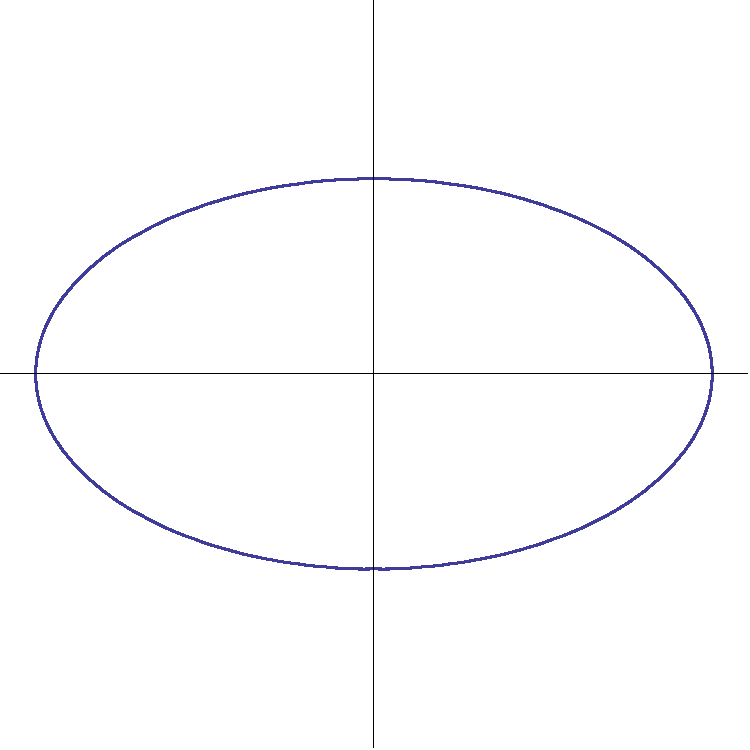
\includegraphics[width = .35\textwidth]{20151202-fig1.pdf}
 \hfil
\begin{picture}(0,0)
\put(0, 86.1){\vector(1, 0){180}}
\put(88.8, 0){\vector(0, 1){175}}
\put(88.8, 86.1){\vector(1, -1){80}}
\put(88.8, 86.1){\line(-1, 1){80}}
\put(88.8, 86.1){\vector(1, 1){80}}
\put(88.8, 86.1){\line(-1, -1){80}}
\put(73, 78){$O$}
\put(182, 83){$x$}
\put(92, 170){$y$}
\put(170, 2){$u$}
\put(170, 166){$v$}
\put(145, 89){$1$}
\put(33, 89){$-1$}
\put(90, 144){$1$}
\put(74, 24){$-1$}
\end{picture}
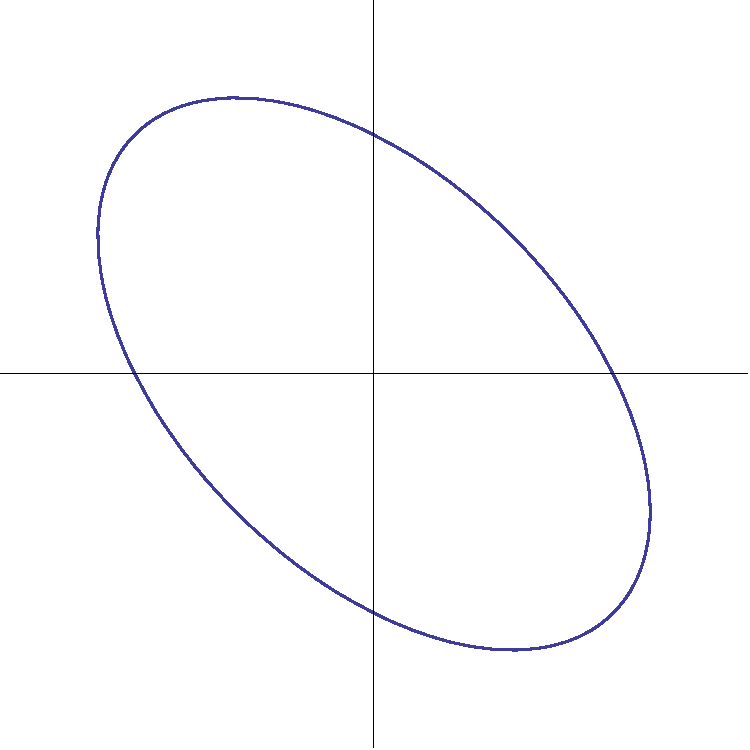
\includegraphics[width = .35\textwidth]{20151202-fig2.pdf}
\end{figure}

\section{おまけ: 双線型写像}

双線型形式とは、一言でいうと「$2$変数の線型写像」のようなものです。今回出てきた標準内積をはじめとして、双線型写像は色々なところに顔を出すので、この機会にいくつか有名な例を見てみましょう。

\subsection{双線型写像}

\paragraph{線型空間の直積} $V, W$を$2$つの線型空間とします。このとき$V$のベクトルと$W$のベクトルのペア全体のなす集合を$V \times W$と書き、$V$と$W$の\textbf{直積}といいます。つまり$V\times W = \{(\bm{v}, \bm{w})\mid \bm{v} \in V, \bm{w} \in W\}$です\footnote{直積は線型空間に限らず、一般に$2$つの集合に対して定義されます。ですが線型空間の直積の場合は
\[
(\bm{v}_1, \bm{w}_1) + (\bm{v}_2, \bm{w}_2) := (\bm{v}_1 + \bm{v}_2, \bm{w}_1, + \bm{w}_2), \quad
\alpha(\bm{v}, \bm{w}) := (\alpha\bm{v}, \alpha\bm{w})
\]
によって和とスカラー倍を定義することで、$V\times W$も線型空間になります。}。

\paragraph{双線型写像の定義}

$U, V, W$を線型空間とします。このとき写像$f\colon U\times V \rightarrow W$で、$1$つ目の変数と$2$つ目の変数の両方について線型なものを\textbf{双線型写像}といいます。すなわち
\[
f(\alpha \bm{u}_1 + \beta \bm{u}_2, \bm{v}) = \alpha f(\bm{u}_1, \bm{v}) + \beta f(\bm{u}_2, \bm{v}), \quad
f(\bm{u}, \alpha \bm{v}_1 + \beta \bm{v}_2) = \alpha f(\bm{u}, \bm{v}_1) + \beta f(\bm{u}, \bm{v}_2)
\]
を満たすものが双線型写像です。特に$U = V$かつ$W = \mathbb{R}$のとき、$\mathbb{R}$に値を取る双線型写像 $f\colon V\times V \rightarrow \mathbb{R}$のことを$V$上の\textbf{双線型形式}といいます。いくつか、典型的な例を見てみましょう。

\paragraph{例1: 行列の積} 

$(m, n)$型行列と$(n, l)$型行列の掛け算をする写像を$m\colon\Mat_{m, n}(\mathbb{R}) \times \Mat_{n, l}(\mathbb{R}) \rightarrow \Mat_{m, l}(\mathbb{R})$とします\footnote{「$(m, n)$型行列」の$m$と線型写像の$m$に同じ文字を使ってしまいましたが、たぶん混ざることはないと思います。}。つまり$m(X, Y) := XY$です。既に行列の積が分配法則などを満たすことを知っているので、任意の$(m, n)$型行列$X, X_1, X_2 \in \Mat_{m, n}(\mathbb{R})$、$Y, Y_1, Y_2 \in \Mat_{n, l}(\mathbb{R})$と実数$\alpha, \beta\in\mathbb{R}$に対し
\begin{align*}
\begin{array}{c@{\,}c@{\,}c@{\,}c@{\,}c@{\,}c@{\,}c}
m(\alpha X_1 + \beta X_2, Y) &=& (\alpha X_1 + \beta X_2)Y &=& \alpha X_1 Y + \beta X_2 Y &=& \alpha\, m(X_1, Y) + \beta\, m(X_2, Y) \\[0.3zw]
m(X, \alpha Y_1 + \beta Y_2) &=& X (\alpha Y_1 + \beta Y_2) &=& \alpha X Y_1 + \beta X Y_2 &=& \alpha\, m(X, Y_1) + \beta\, m(X, Y_2)
\end{array}
\end{align*}
が分かります。よって$m$は双線型写像です。

\paragraph{例2: ベクトルの標準内積} $\bm{u}, \bm{v}\in \mathbb{R}^n$の\textbf{標準内積}$\bm{u}\cdot\bm{v}$を
\[
\bm{u}\cdot\bm{v} := {}^t\bm{u} \bm{v} =
\begin{pmatrix}
u_1 & u_2 & \cdots & u_n 
\end{pmatrix}
\begin{pmatrix}
v_1 \\
v_2 \\
\vdots \\
v_n 
\end{pmatrix}
= u_1 v_1 + u_2 v_2 + \cdots + u_n v_n
\]
と定義しました。この写像は、さっき調べた行列の積を表す写像$m$と行列の転置に分解すれば
\[
\begin{array}{c@{\,}c@{\,}c@{\,}c@{\,}c@{\,}c}
\mathbb{R}^n \times \mathbb{R}^n	& \xrightarrow{\text{\hbox to 3zw{\hfil${}^t \times \id$\hfil}}}	& \Mat_{1, n}(\mathbb{R}) \times \Mat_{n, 1}(\mathbb{R})	& \xrightarrow{\text{\hbox to 3zw{\hfil$m$\hfil}}}	& \Mat_{1, 1}(\mathbb{R})  & = \mathbb{R} \\
\rotatebox{90}{$\in$}	& 																				& \rotatebox{90}{$\in$}										& 													& \rotatebox{90}{$\in$} \\
(\bm{u}, \bm{v})					& \xmapsto{\text{\hbox to 3zw{}}}									& ({}^t\bm{u}, \bm{v})										& \xrightarrow{\text{\hbox to 3zw{}}}				& {}^t\bm{u} \bm{v}
\end{array}
\]
のように、双線型写像と線型写像の合成として表せます。よって全体としても双線型写像だと分かります。

\paragraph{例3: ベクトルの標準内積の一般化} ベクトルの標準内積$(\bm{u}, \bm{v}) \mapsto {}^t\bm{u}\bm{v}$を少し一般化してみます。$n$次正方行列$A \in \Mat_n(\mathbb{R})$を取り、${}^t\bm{u}$と$\bm{v}$の間に$A$を挟んだ$(\bm{u}, \bm{v}) \mapsto {}^t\bm{u} A \bm{v}$という対応を考えます。これもやはり双線型形式です。$A = E$とした場合が、標準内積に対応します。

\paragraph{例4: トレース形式} $(m, n)$型行列$X$と$(n, m)$型行列$Y$のペアに対し$\tr XY$を対応させる写像を考えます。この写像もまた、行列の掛け算の写像を用いると線型写像$\tr$と双線型写像$m$の合成として
\begin{align*}
\begin{array}{c@{\,}c@{\,}c@{\,}c@{\,}c@{\,}c}
\tr\circ m \colon	& \Mat_{m, n}(\mathbb{R}) \times \Mat_{n, m}(\mathbb{R})	& \xrightarrow{\text{\hbox to 3zw{\hfil$m$\hfil}}}	& \Mat_m(\mathbb{R})	& \xrightarrow{\text{\hbox to 3zw{$\hfil\tr$\hfil}}}	& \mathbb{R} \\
					& \rotatebox{90}{$\in$} 									& 													& \rotatebox{90}{$\in$}	& 					& \rotatebox{90}{$\in$} \\
					& (X, Y) 													& \xmapsto{\text{\hbox to 3zw{}}}					& XY					& \xmapsto{\text{\hbox to 3zw{}}}						& \tr XY
\end{array}
\end{align*}
のように書けるので、双線型です。特に$m = n$のとき、この写像は$\Mat_n(\mathbb{R})$上の双線型形式を与えます。

\subsection{内積とノルム}

さて世の中には数多の双線型形式があって、それぞれの性質に応じて用いられる場面は変わってきます。そこで重要な典型例として、僕たちが良く知っている「ベクトルの内積」に焦点を当ててみます。「どういう双線型形式が内積っぽく振る舞うか」を考えてみましょう。

\paragraph{双線型形式の性質} $V$上の対称双線型形式$f$に関する性質を、次のように定義します。
\begin{itemize}
\item 任意の$\bm{v}, \bm{w} \in V$に対し$f(\bm{v}, \bm{w}) = (\bm{w}, \bm{v})$であるとき、$f$は\textbf{対称}であるといいます。
\item 任意の$\bm{v} \in V$に対し$f(\bm{v}, \bm{v}) \geq 0$が成り立つとき、$f$は\textbf{半正定値}であるといいます。
\item $f$が半正定値で、かつ$f(\bm{v}, \bm{v}) = 0$となる$\bm{v} \in V$が$\bm{v} = \bm{0}$しかないとき、$f$は\textbf{正定値}であるといいます。
\end{itemize}
そして$V$上の正定値な対称双線型形式を$V$の\textbf{内積}といいます。また内積のついた線型空間を\textbf{計量線型空間}といいます。。実はこれらの性質が内積を内積たらしめている本質です。さっき挙げた例などをベースに、内積っぽいものを見てみましょう。

\paragraph{例5: $\mathbb{R}^n$の標準内積}

$\mathbb{R}^n$の標準内積は、その名前の指す通り内積になっています。実際${}^t\bm{u}\bm{v} = {}^t\bm{v}\bm{u}$なので、標準内積は対称な双線型形式です。さらに$\bm{v} = {}^t(v_1, v_2, \ldots, v_n)$に対し
\[
\bm{v} \cdot \bm{v} = 
{}^t\bm{v} \bm{v} = 
\begin{pmatrix}
v_1 & v_2 & \cdots & v_n
\end{pmatrix}
\begin{pmatrix}
v_1 \\
v_2 \\
\vdots \\
v_n
\end{pmatrix}
= v_1^2 + v_2^2 + \cdots + v_n^2 \geq 0
\]
で、この値が$0$になるのは$\bm{v} = \bm{0}$のときに限ります。よって標準内積は正定値でもあります。

\paragraph{例6: 行列の内積} トレース形式に行列の転置をかませて
\begin{align*}
\begin{array}{c@{\,}c@{\,}c@{\,}c@{\,}c@{\,}c@{\,}c}
\Mat_{m, n}(\mathbb{R}) \times \Mat_{m, n}(\mathbb{R})	& \xrightarrow{\text{\hbox to 3zw{\hfil${}^t \times \id$\hfil}}}	& \Mat_{n, m}(\mathbb{R}) \times \Mat_{m, n}(\mathbb{R})	& \xrightarrow{\text{\hbox to 3zw{\hfil$m$\hfil}}}	& \Mat_n(\mathbb{R})	& \xrightarrow{\text{\hbox to 3zw{\hfil$\tr$\hfil}}}	& \mathbb{R} \\
\rotatebox{90}{$\in$}									& 																	& \rotatebox{90}{$\in$}										& 													& \rotatebox{90}{$\in$}	&		 												& \rotatebox{90}{$\in$} \\
(A, B)													& \xmapsto{\text{\hbox to 3zw{}}}						& ({}^t\!A, B)												& \xmapsto{\text{\hbox to 3zw{}}}			& {}^t\!A B				& \xmapsto{\text{\hbox to 3zw{}}}			& \tr({}^t\!A B)
\end{array}
\end{align*}
という双線型形式を考えます。これを成分で書き下してみましょう。$A = (a_{ij})$, $B = (b_{ij}) \in \Mat_{m, n}(\mathbb{R})$とすると
\begin{align*}
& {}^t\!A B 
=
\begin{pmatrix}
a_{11} & a_{21} & \cdots & a_{m1} \\
a_{12} & a_{22} & \cdots & a_{m2} \\
\vdots & \vdots & \ddots & \vdots \\
a_{1n} & a_{2n} & \cdots & a_{mn}
\end{pmatrix}
\begin{pmatrix}
b_{11} & b_{12} & \cdots & b_{1n} \\
b_{21} & b_{22} & \cdots & b_{2n} \\
\vdots & \vdots & \ddots & \vdots \\
b_{m1} & b_{m2} & \cdots & b_{mn}
\end{pmatrix} \\
&=
\begin{pmatrix}
a_{11}b_{11} + a_{21}b_{21} + \cdots + a_{m1}b_{m1} & * & \cdots & * \\
* & a_{12}b_{12} + a_{22}b_{22} + \cdots + a_{m2}b_{m2} & \cdots & * \\
\vdots & \vdots & \ddots & \vdots \\
* & * & \cdots & a_{1n}b_{1n} + a_{2n}b_{2n} + \cdots + a_{mn}b_{mn}
\end{pmatrix}
\end{align*}
です\footnote{この後トレースを取るので、非対角成分の計算は不要です。どうでもいい成分を$*$で表しました。}。よって
\[
\tr {}^t\!A B
= (a_{11}b_{11} + a_{21}b_{21} + \cdots + a_{m1}b_{m1}) + \cdots + (a_{1n}b_{1n} + a_{2n}b_{2n} + \cdots + a_{mn}b_{mn})
= \sum_{i = 1}^{m} \sum_{j = 1}^n a_{ij}b_{ij}
\]
となります。この内積は「対応する成分同士を掛け算して足し合わせる」という計算をしていますから、$\mathbb{R}^n$の標準内積を行列バージョンに拡張したものだと思うことができます。実際この式で$n = 1$とすれば、$\mathbb{R}^m$の標準内積が再現されますね。そして標準内積の時と同様、特に$A = B$とすると
\[
\tr {}^t\!A A = (a_{11}^2 + a_{21}^2 + \cdots + a_{m1}^2) + \cdots + (a_{1n}^2 + a_{2n}^2 + \cdots + a_{mn}^2) \geq 0
\]
で、等号成立は$A = O$のときに限ります。こうして行列の空間$\Mat_{m, n}(\mathbb{R})$に、標準内積と呼ぶべきものを定義できました。

\paragraph{ノルムと距離} 線型空間$V$上に内積$(, )$が与えられたとします。このとき任意の$\bm{v} \in V$に対し$(\bm{v}, \bm{v}) \geq 0$が成り立つので、$\|\bm{v}\| := \sqrt{(\bm{v}, \bm{v})}$が定義できます。これを$\bm{v}$の\textbf{ノルム}といいます。ノルムは
\begin{itemize}
\item 任意の$\bm{v} \in V$に対し$\|\bm{v}\|\geq 0$で、かつ$\|\bm{v}\| = 0$となる$\bm{v}$は$\bm{v} = \bm{0}$に限る
\item 任意の$\bm{v} \in V$と$\alpha\in\mathbb{R}$に対し、$\|\alpha\bm{v}\| = |\alpha|\|\bm{v}\|$が成り立つ
\item 任意の$\bm{u}, \bm{v} \in V$に対し、$\|\bm{u} + \bm{v}\| \leq \|\bm{u}\| + \|\bm{v}\|$が成り立つ
\end{itemize}
という性質を満たします\footnote{内積とは関係なく、一般に今の$3$条件を満たす写像$\|\ \|\colon V\rightarrow\mathbb{R}_{\geq 0}$はノルムと呼ばれます。}。さらにノルムがあると、$\bm{u}, \bm{v} \in V$に対し$d(\bm{u}, \bm{v}) := \|\bm{u} - \bm{v}\|$によって$V$上の\textbf{距離}が定義できます。この$d$を距離というのは
\begin{itemize}
\item 任意の$\bm{u}, \bm{v} \in V$に対して$d(\bm{u}, \bm{v}) \geq 0$
\item 任意の$\bm{u}, \bm{v} \in V$に対して$d(\bm{u}, \bm{v}) = 0$ならば$\bm{u} = \bm{v}$
\item 任意の$\bm{u}, \bm{v} \in V$に対して$d(\bm{u}, \bm{v}) = d(\bm{v}, \bm{u})$
\item 任意の$\bm{u}, \bm{v}, \bm{w} \in V$に対して$d(\bm{u}, \bm{v}) \leq d(\bm{u}, \bm{w}) +d(\bm{w}, \bm{v})$ (三角不等式)
\end{itemize}
という、いかにも距離と呼ぶにふさわしい性質が成り立つからです。確かめてみてください。

ちなみに内積に限らずとも、今挙げたような意味での「距離」が備わった空間を\textbf{距離空間}といいます\footnote{距離空間は線型空間である必要はありまえん。たとえば$\mathbb{R}^2$内の原点を中心とする半径$1$の開円板なども、距離空間の例です。}。またノルムの定義された線型空間を\textbf{ノルム空間}といいます\footnote{いまは内積を出発点にしてしまいましたが、「計量線型空間にはなり得ないノルム空間」の存在が知られています。}。したがって
\[
\text{計量線型空間} \Longrightarrow
\text{ノルム空間} \Longrightarrow
\text{距離空間}
\]
という関係が成り立ちます。

\subsection{Hermite形式}

$\mathbb{R}^n$の標準内積を真似ることで、複素数を変数とする$2$本の$n$次元数ベクトル$\bm{u}, \bm{v} \in \mathbb{C}^n$に対しても、$(\bm{u}, \bm{v})\mapsto {}^t\bm{u} \bm{v}$という双線型形式を考えることができます。ですが既に述べたように、この双線型形式は、ある意味振る舞いが良くありません\footnote{以下で述べるように、ここで「振る舞いが良くない」と言っているのはあくまで「複素線型空間上でノルムを作りたいなら、双線型形式ではダメだよね」というだけの話です。双線型形式は双線型形式で、別の場面で役立ちます。たとえば$\mathfrak{sl}_2(\mathbb{C})$上のトレース形式に適当な定数をかけるとKilling形式というものになり、Lie環の理論で非常に重要な役割を果たします。}。$\mathbb{R}^n$の内積では「ノルムを経由して長さや距離が定義できる」というご利益がありましたが、$\mathbb{C}^n$の場合にはそういうことが起きません。そこでベクトルの片方に複素共役をつけて$f(\bm{u}, \bm{v}) := {}^t\bm{u}\overline{\bm{v}}$と書くと、$f$は
\begin{itemize}
\item $f(\alpha \bm{u}_1 + \beta \bm{u}_2, \bm{v}) = \alpha f(\bm{u}_1, \bm{v}) + \beta f(\bm{u}_2, \bm{v}) $
\item $f(\bm{v}, \bm{u}) = \overline{f(\bm{u}, \bm{v})}$
\item 任意の$\bm{u} \in \mathbb{C}^n$に対し、$f(\bm{u}, \bm{u}) \in \mathbb{R}_{\geq 0}$
\item $f(\bm{u}, \bm{u}) = 0$ならば$\bm{u} = \bm{0}$
\end{itemize}
という式を満たすようになります。これを実ベクトル空間の内積と見比べると、
\begin{itemize}
\item 正定値という性質は保たれている
\item 双線型性と対称性が若干崩れ、式に複素共役が混ざる
\end{itemize}
ということが分かります。双線型性や対称性を若干犠牲にしたことと引き換えに、正定値性が得られたわけです。このような式を満たす$f$を\textbf{Hermite形式}といいます。複素線型空間$V$上にHermite形式$(, )$が与えられると、実線型空間の時と同様$\|\bm{v}\| := \sqrt{(\bm{v}, \bm{v})}$によって$\bm{v} \in V$のノルムが定義できます。

\subsection{ノルムの応用: 行列の指数函数}

せっかくノルムを定義したので、一つ使い道を紹介しましょう。それは\textbf{行列の指数函数}というものです。

普通の数に対する指数函数$e^x = \exp x$は\footnote{$e^x$と$\exp x$は全く同じ意味です。$x$の部分に長い式が来る場合、$e$の肩に載せると見辛くなるので、$\exp$という記法が用いられます。}、Taylor展開を用いて
\[
e^x = \sum_{k = 0}^{\infty} \frac{x^k}{k!} = 1 + x + \frac{x^2}{2!} + \frac{x^3}{3!} + \cdots
\]
と表示できます。この$x$に行列を代入できないでしょうか?

一つの戦略としては「代入する行列を制限する」という手があります。$e^x$の$x$のところに巾零行列を代入すると、右辺は有限項で終わってしまうので、定義通りに計算ができます。

もう一つの戦略としては「収束を検討する」というものです。数列の収束を拡張して、「行列の列」の収束を「各成分が収束すること」と定めれば、行列の列の極限を考えることができます。それを使って指数函数$e^x$を行列に拡張します。この時に活躍するのが、行列のノルムです\footnote{なお、以下の証明では、行列の成分は実数でも複素数でも構いません。}。

\paragraph{行列の収束とトレースノルム}

いま$n$次正方行列の列$(A_k)_{k = 0}^{\infty}$と$A$について、$A_n \rightarrow A$ ($n\rightarrow\infty$) を「$A_n$の各成分が、$n \rightarrow \infty$で同じ場所にある$A$の成分に収束すること」と定めました。実はこの条件は、トレースノルム$\|A\| := \tr {}^t\!A A$を使うと$\|A_n - A\| \rightarrow 0$と簡単に書けてしまいます。このことを証明しましょう。$A_k = \bigl(a^{(k)}_{ij}\bigr)$, $A = (a_{ij})$と書きます。

まず$A_k \rightarrow A$とします。このとき全ての$1 \leq i, j \leq n$に対し$|a^{(k)}_{ij} - a_{ij}| \rightarrow 0$が成り立つので、
\begin{align*}
\lim_{k \rightarrow \infty} \|A_k - A\|
&= \lim_{k \rightarrow \infty} \sum_{i, j = 0}^n |a^{(k)}_{ij} - a_{ij}|^2 
= \sum_{i, j = 0}^n \lim_{k \rightarrow \infty} |a^{(k)}_{ij} - a_{ij}|^2 
= 0
\end{align*}
となります。逆に$\|A_k - A\| \rightarrow 0$とすると、任意の$1\leq p, q\leq n$に対し
\begin{align*}
0
\leq \bigl| a^{(k)}_{pq} - a_{pq} \bigr|^2
\leq \sum_{i, j = 0}^n \bigl| a^{(k)}_{ij} - a_{ij} \bigr|^2
= \|A_k - A\|
\rightarrow 0 \quad (k \rightarrow \infty)
\end{align*}
となるから、各成分毎の収束が言えます。こんな感じで、行列の収束の話がノルムの計算に帰着できるのです。

また、ノルムの列$\bigl(\|A_k\|\bigr)_{k = 0}^{\infty}$がCauchy列なら、$(A_k)_{k = 0}^{\infty}$が収束すると言えます。今の評価と同様にして、任意の自然数$m, m'\in\mathbb{N}$に対し$|A^{(m)}_{ij} - A^{(m')}_{ij}| \leq \|A_m - A_{m'}\|$が示せます。つまり全ての成分について「第$m$番目と第$m'$番目の項の差がノルム$\|A_m - A_{m'}\|$で抑えられる」というわけです。よってノルムの列$\bigl(\|A_k\|\bigr)_{k = 0}^{\infty}$がCauchy列になっていたら、$(A_k)_{k = 0}^{\infty}$もCauchy列となり、収束します。


\paragraph{トレースノルムの満たす不等式}

次に、トレースノルムについて$\|AB\| \leq \|A\| \|B\|$が成り立つことを示しましょう。${}^t\!A = (\bm{a}_1 \ \cdots \ \bm{a}_n)$, $B = (\bm{b}_1, \ldots, \bm{b}_n)$とすると、
\[
AB =
\begin{pmatrix}
{}^t\bm{a}_1 \\
{}^t\bm{a}_2 \\
\vdots \\
{}^t\bm{a}_n
\end{pmatrix}
\begin{pmatrix}
\bm{b}_1 & \bm{b}_2 & \cdots & \bm{b}_n
\end{pmatrix}
=
\begin{pmatrix}
\bm{a}_1 \cdot \bm{b}_1 & \bm{a}_1 \cdot \bm{b}_2 & \cdots & \bm{a}_1 \cdot \bm{b}_n \\
\bm{a}_2 \cdot \bm{b}_1 & \bm{a}_2 \cdot \bm{b}_2 & \cdots & \bm{a}_2 \cdot \bm{b}_n \\
\vdots & \vdots & \ddots & \vdots \\
\bm{a}_n \cdot \bm{b}_1 &  \bm{a}_n \cdot \bm{b}_2 & \cdots & \bm{a}_n \cdot \bm{b}_n
\end{pmatrix}
\]
なので、Cauchy--Schwarzの不等式$|\bm{a}\cdot\bm{b}| \leq \|\bm{a}\| \|\bm{b}\| $を使うと
\begin{align*}
\|AB\|
&= \sum_{i, j = 1}^n |\bm{a}_i \cdot \bm{b}_j|^2
\leq \sum_{i, j = 1}^n \|\bm{a}_i\|^2 \|\bm{b}_j\|^2
= \Biggl(\sum_{i = 1}^n \|\bm{a}_i\|^2 \Biggr) \Biggl( \sum_{j = 1}^n \|\bm{b}_j\|^2 \Biggr)
= \|A\| \|B\|
\end{align*}
となります。

\paragraph{指数函数が収束すること}

ここまで来れば、あとは簡単です。ノルムが三角不等式と$\|AB\| \leq \|A\| \|B\|$を満たすことから、$m \geq l \geq 0$に対し
\begin{align*}
\Biggl\|\sum_{k = 0}^m \frac{A^k}{k!} - \sum_{k = 0}^l \frac{A^k}{k!} \Biggr\|
= \Biggl\|\sum_{k = l + 1}^m \frac{A^k}{k!} \Biggr\|
\leq \sum_{k = l + 1}^m \biggl\|\frac{A^k}{k!} \biggr\|
\leq \sum_{k = l + 1}^m \frac{\|A^k\|}{k!}
\leq \sum_{k = l + 1}^m \frac{\|A\|^k}{k!}
\end{align*}
となります。ここで指数函数$e^x$をTaylor展開して得られる級数の収束半径が$\infty$だったことを思い出しましょう。収束列であることとCauchy列であることは同値なので、数列$\bigl(\sum_{k = 0}^m \frac{\|A\|^k}{k!}\bigr)_{m = 0}^{\infty}$はCauchy列になっています。よってノルムの列$\bigl(\|\sum_{k = 0}^m \frac{A^k}{k!}\|\bigr)_{m = 0}^{\infty}$もCauchy列になるので、$\sum_{k = 0}^{\infty} A^k / k!$の収束が言えました。$e^x$の収束半径が$\infty$なので、全ての行列$A$に対して収束が言えます。これで行列の指数函数を定義できました。

\paragraph{指数函数の使い道}

さて、せっかく行列の指数函数を定義したので、その使い道を$1$つ紹介しましょう。それは微分方程式です。$a \in \mathbb{R}$のとき、$t$の函数$y(t)$に関する微分方程式
\[
y' = ay
\]
という微分方程式の解が$y = e^{at} y(0)$という形に書けることは、既に知っているはずです。これをちょっと拡張して、行列の形で書かれた微分方程式
\[
\begin{pmatrix}
y_1' \\
y_2'
\end{pmatrix}
=
\begin{pmatrix}
a & c \\
b & d
\end{pmatrix}
\begin{pmatrix}
y_1 \\
y_2
\end{pmatrix}
\]
を考えてみましょう。これをベクトルと行列で$\bm{y}' = A \bm{y}$と書くと、行列の指数函数で$\bm{y} = e^{tA} \bm{y}(0)$と書ける予感がしてきます。実際それは正しく、この問題のような定数係数の連立線型微分方程式は、行列の指数函数を使うと解くことができます。さらに行列の指数函数は$P^{-1} e^{A} P = e^{P^{-1} A P}$という式を満たすので、指数函数の肩に乗せる行列をJordan標準形に直しておくことで計算ができます。こんな風にして、線型代数の理論は微分方程式を解くのにも役立てられるのです。

